\subsubsection{Checkout}
\label{UseCase_Checkout}

\paragraph{Kurzbeschreibung}
   Ein \Gls{Gast} der ein \Gls{Zimmer} bezogen hat kommt zur \Gls{Rezeption}.
   Der \Gls{Rezeptionist} sucht die Daten des \Gls{Gast}es. Mit diesen Daten
   werden sämtliche \Glspl{Arrangement} und in Anspruch genommene
   Leistungen aufgelistet und damit eine \Gls{Zwischenrechnung} erstellt.
   Dem \Gls{Gast} wird diese ausgehändigt. Nach Kontrolle der
   \Gls{Zwischenrechnung} wird die Zahlungsart und Modalitäten ausgehandelt.
   Sobald der \Gls{Gast} die \Gls{Rechnung} beglichen  hat wird eine endgültige
   Rechnung ausgedruckt und dem \Gls{Gast} übergeben.
   Nach dem  Bezahlen der \Gls{Rechnung} registriert das System dass der
   \Gls{Gast} abgereist ist.

\paragraph{Stakeholders und Akteure}
\begin{itemize}
	\item \Gls{Rezeptionist} - Schnelle und zuverlässige Bearbeitung des
	\Gls{Checkout}s, Konzentration auf den \Gls{Gast}, nicht auf den Bildschirm
	\item \Gls{Gast} - möchte einen reibungslosen, zügigen Ablauf und so schnell
	wie möglich abreisen
\end{itemize}

\paragraph{Vorbedingung}
\begin{itemize}
	\item Gast muss im System eingecheckt sein
\end{itemize}

\paragraph{Nachbedingung}
\begin{itemize}
	\item Die Rechnung muss an die Buchhaltung übergeben werden können
	\item Das Zimmer muss im System wieder als frei markiert sein
\end{itemize}

\paragraph{Basisablauf}
\begin{enumerate}
	\item Eine Person kommt zum \Gls{Rezeption} und gibt seine \Gls{Zimmernummer} an.
	\item Der \Gls{Rezeptionist} sucht im System anhand der \Gls{Zimmernummer} den \Gls{Gast}.
	\item Das System zeigt die in Anspruch genommene Leistungen an.
    \item Das System erstellt eine \Gls{Zwischenrechnung}.
	\item Der \Gls{Gast} kontrolliert die \Gls{Zwischenrechnung}.
	\item Der \Gls{Gast} erhält vom System die endgültige \Gls{Rechnung}.
	\item Der \Gls{Gast} bezahlt die \Gls{Zwischenrechnung}.
	\item Der \Gls{Rezeptionist} teilt dem System mit, dass der \Gls{Gast} wieder abgereist ist.
	\item Der \Gls{Gast} gibt den Schlüssel ab.
\end{enumerate}

\paragraph{Alternativer Ablauf}
\begin{longenum}
	\item
	\begin{longenum}
		\item Der \Gls{Gast} kennt seine \Gls{Zimmernummer} nicht:
		\begin{longenum}
			\item Der \Gls{Gast} gibt stattdessen seinen Namen an.
			\item Der \Gls{Rezeptionist} sucht die \Gls{Zimmernummer} im System anhand des	Namens.
			\item \emph{weiter mit Basisablauf Punkt 3}
		\end{longenum}
	\end{longenum}
	\item
	\item
	\item
	\item
	\begin{longenum}
		\item Der \Gls{Gast} ist mit der \Gls{Zwischenrechnung} nicht einverstanden:
		\begin{longenum}
			\item Der \Gls{Rezeptionist} holt den Geschäftsführer
			\item Nachdem einige Rechnungspunkte besprochen wird eine neue Rechnung
			erstellt.
			\item \emph{weiter mit Basisablauf Punkt 6}
		\end{longenum}
	\end{longenum}
	\begin{longenum}
	\item Der \Gls{Gast} will bestimmte Rechnungspostionen auf einer eigenen
	\Gls{Rechnung}:
		\begin{longenum}
			\item Der \Gls{Rezeptionist} nimmt die gewünschten Rechnungspositionen von
			der \Gls{Zwischenrechnung} und erstellt mit Ihnen eine eigene \Gls{Rechnung}.
			\item Der \Gls{Gast} kontrolliert die neuen \Gls{Rechnung}en und nimmts sie
			entgegen.
			\item \emph{weiter mit Basisablauf Punkt 6}
		\end{longenum}
	\end{longenum}
	\begin{longenum}
	\item Der \Gls{Gast} will das die Rechnung auf eine andere Person lautet:
		\begin{longenum}
			\item Der \Gls{Rezeptionist} trägt die angegebenen Daten als \Gls{Kunde} ein.
			\item \emph{weiter mit Basisablauf Punkt 6}
		\end{longenum}
	\end{longenum}
	\item
	\item
	\begin{longenum}
		\item Der \Gls{Kunde} will die Rechnung nicht gleich bezahlen:
		\begin{longenum}
			\item Der \Gls{Rezeptionist} vergewissert sich das der \Gls{Gast} auf Kredit
			zahlen kann.
			\begin{longenum}
				\item Der \Gls{Gast} kann nicht auf Kredit bezahlen:
				\begin{longenum}
					\item Der \Gls{Rezeptionist} macht den Kunden darauf aufmerksam.
					\item \emph{weiter mit Basisablauf Punkt 7}
				\end{longenum}
			\end{longenum}
			\begin{longenum}
				\item Der \Gls{Gast} kann auf Kredit bezahlen:
				\begin{longenum}
					\item Der \Gls{Rezeptionist} ändert die Zahlungsart der \Gls{Rechnung} auf
					Kredit.
					\item \emph{weiter mit Basisablauf Punkt 8}.
				\end{longenum}
			\end{longenum}
		\end{longenum}
	\end{longenum}
	\item
	\item
	\begin{longenum}
		\item Der \Gls{Gast} hat den Zimmerschlüssel verloren:
		\begin{longenum}
			\item Der \Gls{Rezeptionist} teilt dem System den Verlust des Schlüssels mit.
			\item Der \Gls{Gast} muss eine Entschädigung für den Verlust leisten.
		\end{longenum}
	\end{longenum}
\end{longenum}

\paragraph{Sequenzdiagramm}
:\\
\begin{figure}[h]
	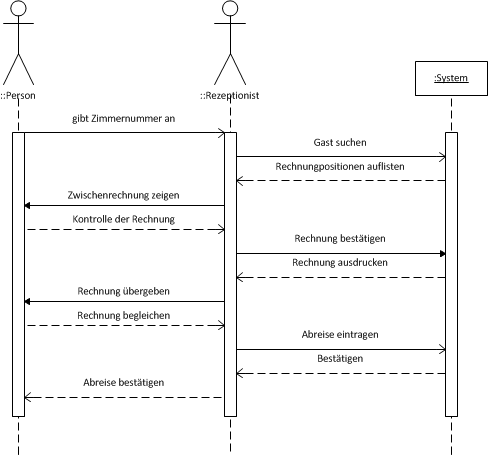
\includegraphics{Images/SSD_Checkout.png}
	\caption{Checkout - Sequenzdiagramm}
\end{figure}
\paragraph{Besondere Anforderungen}
\begin{itemize}
	\item keine
\end{itemize}

\paragraph{Benutzerfrequenz}
mehrmals täglich (sehr hoch)

\paragraph{Offene Punkte}

\newpage
